\documentclass{standalone}
\usepackage{tikz}
\usetikzlibrary{patterns, positioning}
\usepackage[sfdefault]{ClearSans} %% option 'sfdefault' activates Clear Sans as the default text font
\usepackage[T1]{fontenc}

\begin{document}
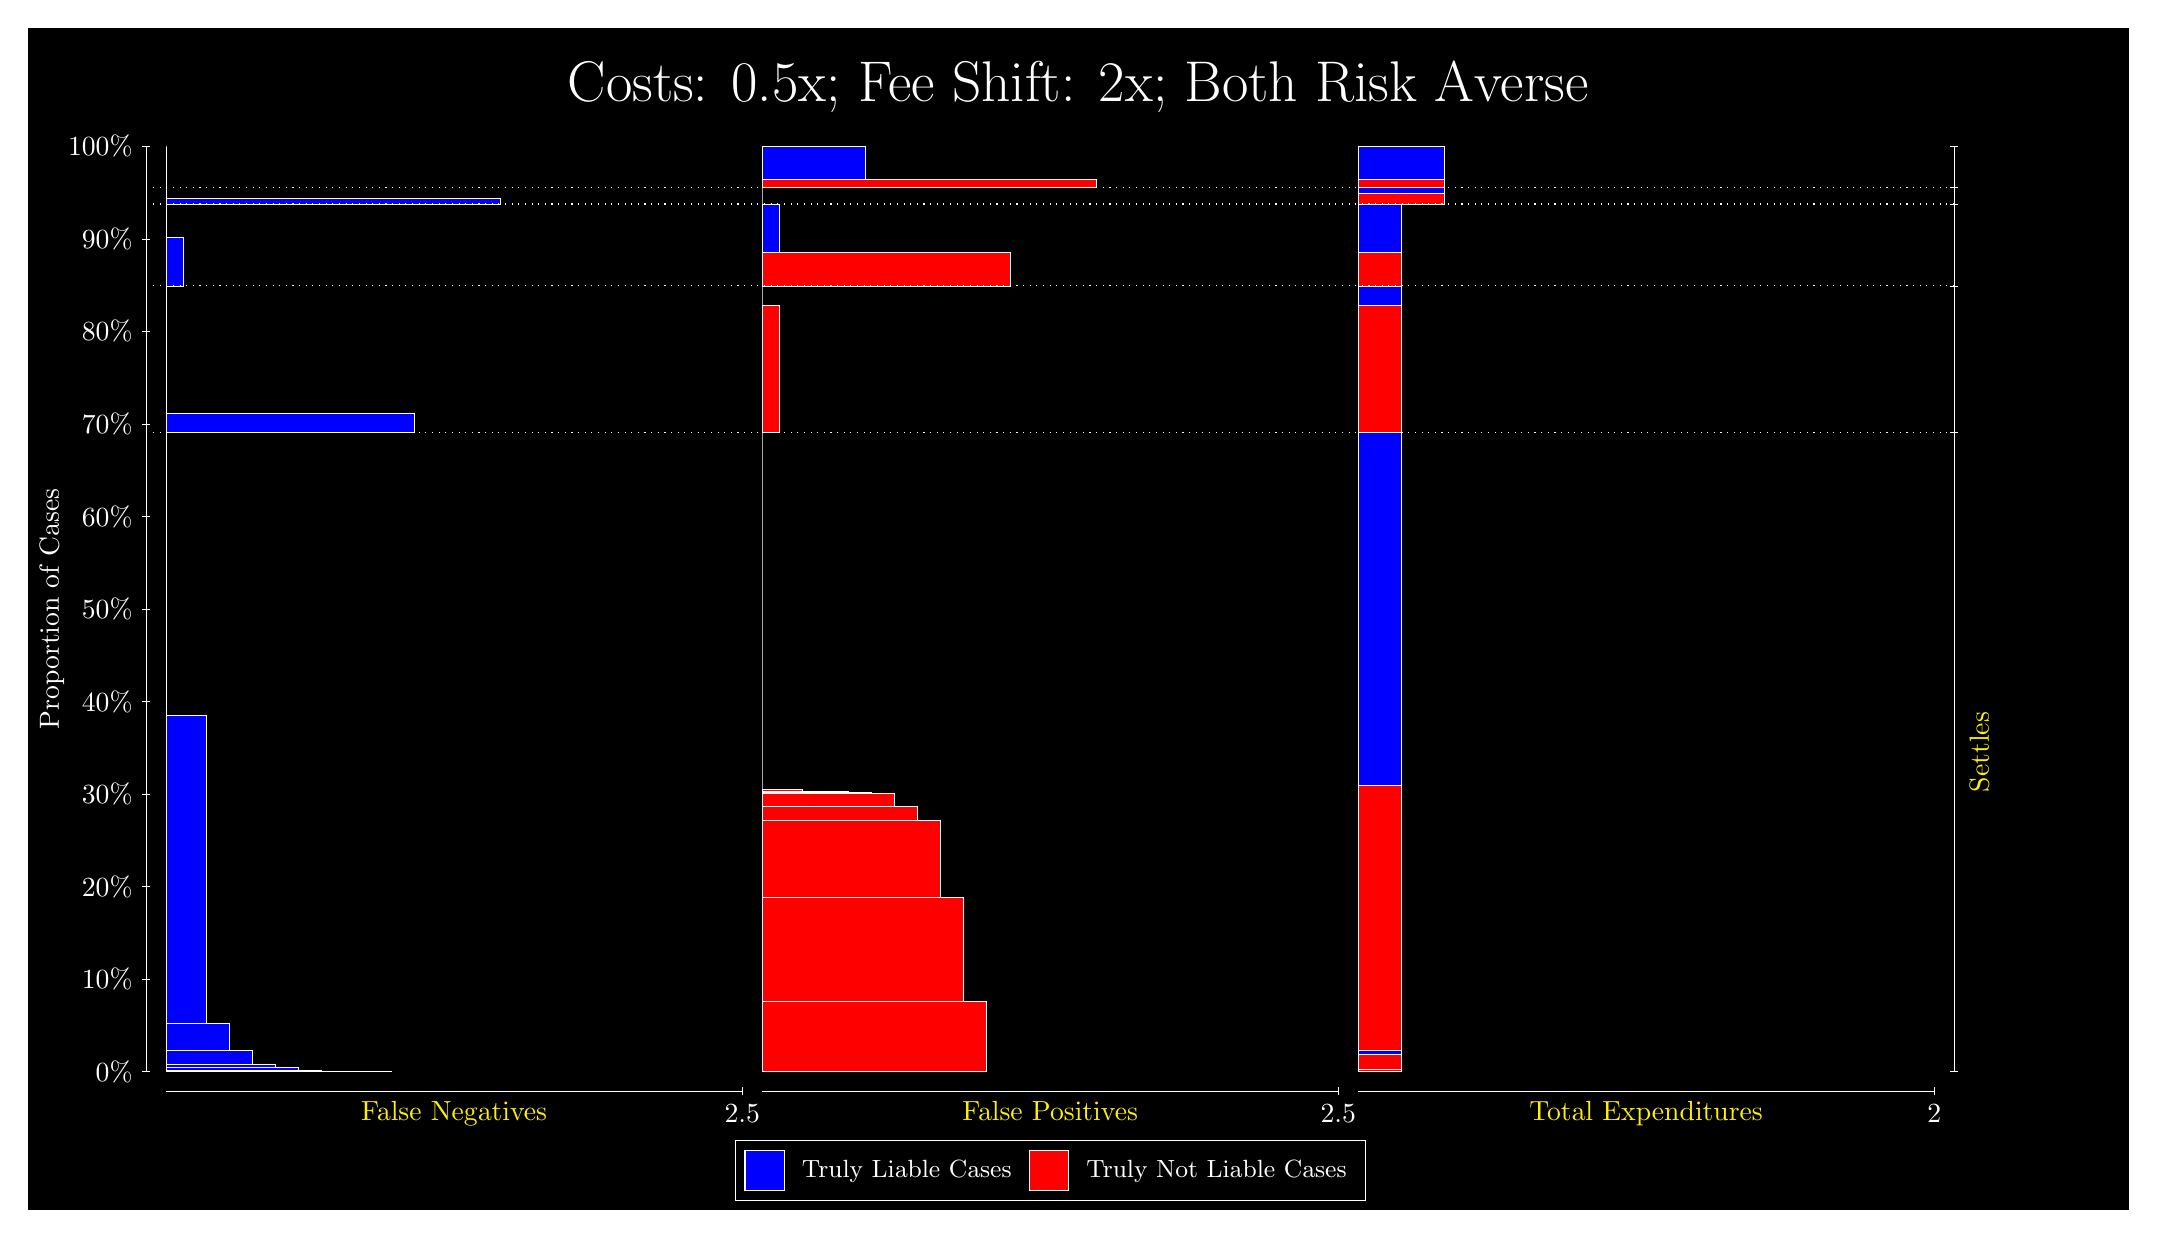
\begin{tikzpicture}
\draw[fill=black] (0,0) rectangle (26.667,15);
\draw[text=white] (0,13.5) rectangle (26.667,15) node[midway] {\huge Costs: 0.5x; Fee Shift: 2x; Both Risk Averse};
\draw[white, very thin] (1.5,1.75) -- (1.5,13.5);
\node[rotate=90, text=white, anchor=center] at (0.3, 7.625) {Proportion of Cases};
\draw[white, very thin] (1.45,1.75) -- (1.55,1.75);
\node[text=white, anchor=east] at (1.45, 1.75) {0\%};
\draw[white, very thin] (1.45,2.925) -- (1.55,2.925);
\node[text=white, anchor=east] at (1.45, 2.925) {10\%};
\draw[white, very thin] (1.45,4.1) -- (1.55,4.1);
\node[text=white, anchor=east] at (1.45, 4.1) {20\%};
\draw[white, very thin] (1.45,5.275) -- (1.55,5.275);
\node[text=white, anchor=east] at (1.45, 5.275) {30\%};
\draw[white, very thin] (1.45,6.45) -- (1.55,6.45);
\node[text=white, anchor=east] at (1.45, 6.45) {40\%};
\draw[white, very thin] (1.45,7.625) -- (1.55,7.625);
\node[text=white, anchor=east] at (1.45, 7.625) {50\%};
\draw[white, very thin] (1.45,8.8) -- (1.55,8.8);
\node[text=white, anchor=east] at (1.45, 8.8) {60\%};
\draw[white, very thin] (1.45,9.975) -- (1.55,9.975);
\node[text=white, anchor=east] at (1.45, 9.975) {70\%};
\draw[white, very thin] (1.45,11.15) -- (1.55,11.15);
\node[text=white, anchor=east] at (1.45, 11.15) {80\%};
\draw[white, very thin] (1.45,12.325) -- (1.55,12.325);
\node[text=white, anchor=east] at (1.45, 12.325) {90\%};
\draw[white, very thin] (1.45,13.5) -- (1.55,13.5);
\node[text=white, anchor=east] at (1.45, 13.5) {100\%};

\draw[white, very thin] (24.457,1.75) -- (24.457,13.5);
\draw[white, very thin] (24.407,1.75) -- (24.507,1.75);
\node[anchor=west] at (24.407, 1.75) {};
\draw[white, very thin] (24.407,9.8658) -- (24.507,9.8658);
\node[anchor=west] at (24.407, 9.8658) {};
\draw[white, very thin] (24.407,11.728) -- (24.507,11.728);
\node[anchor=west] at (24.407, 11.728) {};
\draw[white, very thin] (24.407,12.767) -- (24.507,12.767);
\node[anchor=west] at (24.407, 12.767) {};
\draw[white, very thin] (24.407,12.982) -- (24.507,12.982);
\node[anchor=west] at (24.407, 12.982) {};
\draw[white, very thin] (24.407,13.5) -- (24.507,13.5);
\node[anchor=west] at (24.407, 13.5) {};

\draw[white, very thin, fill=blue] (1.75,1.75) rectangle (4.6044,1.7553);
\draw[white, very thin, fill=blue] (1.75,1.7553) rectangle (4.3116,1.7561);
\draw[white, very thin, fill=blue] (1.75,1.7561) rectangle (4.0188,1.7587);
\draw[white, very thin, fill=blue] (1.75,1.7587) rectangle (3.7261,1.7626);
\draw[white, very thin, fill=blue] (1.75,1.7626) rectangle (3.4333,1.8002);
\draw[white, very thin, fill=blue] (1.75,1.8002) rectangle (3.1406,1.8409);
\draw[white, very thin, fill=blue] (1.75,1.8409) rectangle (2.8478,2.0226);
\draw[white, very thin, fill=blue] (1.75,2.0226) rectangle (2.5551,2.3629);
\draw[white, very thin, fill=blue] (1.75,2.3629) rectangle (2.2623,6.2801);
\draw[white, very thin, fill=red] (1.75,6.2801) rectangle (1.75,9.8658);
\draw[white, very thin, fill=blue] (1.75,9.8658) rectangle (4.8971,10.109);
\draw[white, very thin, fill=red] (1.75,10.109) rectangle (1.75,11.728);
\draw[white, very thin, fill=blue] (1.75,11.728) rectangle (1.9696,12.342);
\draw[white, very thin, fill=red] (1.75,12.342) rectangle (1.75,12.767);
\draw[white, very thin, fill=blue] (1.75,12.767) rectangle (5.9949,12.84);
\draw[white, very thin, fill=red] (1.75,12.84) rectangle (1.75,12.982);
\draw[white, very thin, fill=red] (1.75,12.982) rectangle (1.75,13.086);
\draw[white, very thin, fill=blue] (1.75,13.086) rectangle (1.75,13.5);
\draw[white, very thin, fill=red] (9.3189,1.75) rectangle (12.173,2.6361);
\draw[white, very thin, fill=red] (9.3189,2.6361) rectangle (11.88,3.9636);
\draw[white, very thin, fill=red] (9.3189,3.9636) rectangle (11.588,4.9437);
\draw[white, very thin, fill=red] (9.3189,4.9437) rectangle (11.295,5.1218);
\draw[white, very thin, fill=red] (9.3189,5.1218) rectangle (11.002,5.2881);
\draw[white, very thin, fill=red] (9.3189,5.2881) rectangle (10.709,5.2918);
\draw[white, very thin, fill=red] (9.3189,5.2918) rectangle (10.709,5.2994);
\draw[white, very thin, fill=red] (9.3189,5.2994) rectangle (10.417,5.3077);
\draw[white, very thin, fill=red] (9.3189,5.3077) rectangle (10.124,5.3115);
\draw[white, very thin, fill=red] (9.3189,5.3115) rectangle (9.8312,5.3356);
\draw[white, very thin, fill=blue] (9.3189,5.3356) rectangle (9.3189,9.8658);
\draw[white, very thin, fill=red] (9.3189,9.8658) rectangle (9.5384,11.485);
\draw[white, very thin, fill=blue] (9.3189,11.485) rectangle (9.3189,11.728);
\draw[white, very thin, fill=red] (9.3189,11.728) rectangle (12.466,12.153);
\draw[white, very thin, fill=blue] (9.3189,12.153) rectangle (9.5384,12.767);
\draw[white, very thin, fill=red] (9.3189,12.767) rectangle (9.3189,12.909);
\draw[white, very thin, fill=blue] (9.3189,12.909) rectangle (9.3189,12.982);
\draw[white, very thin, fill=red] (9.3189,12.982) rectangle (13.564,13.086);
\draw[white, very thin, fill=blue] (9.3189,13.086) rectangle (10.636,13.5);
\draw[white, very thin, fill=red] (16.888,1.75) rectangle (17.437,1.7734);
\draw[white, very thin, fill=blue] (16.888,1.7734) rectangle (17.437,1.7807);
\draw[white, very thin, fill=red] (16.888,1.7807) rectangle (17.437,1.9712);
\draw[white, very thin, fill=blue] (16.888,1.9712) rectangle (17.437,2.014);
\draw[white, very thin, fill=red] (16.888,2.014) rectangle (17.437,5.3859);
\draw[white, very thin, fill=blue] (16.888,5.3859) rectangle (17.437,9.8658);
\draw[white, very thin, fill=red] (16.888,9.8658) rectangle (17.437,11.485);
\draw[white, very thin, fill=blue] (16.888,11.485) rectangle (17.437,11.728);
\draw[white, very thin, fill=red] (16.888,11.728) rectangle (17.437,12.153);
\draw[white, very thin, fill=blue] (16.888,12.153) rectangle (17.437,12.767);
\draw[white, very thin, fill=red] (16.888,12.767) rectangle (17.986,12.909);
\draw[white, very thin, fill=blue] (16.888,12.909) rectangle (17.986,12.982);
\draw[white, very thin, fill=red] (16.888,12.982) rectangle (17.986,13.086);
\draw[white, very thin, fill=blue] (16.888,13.086) rectangle (17.986,13.5);
\draw[white, dotted] (1.5,9.8658) -- (24.457,9.8658);
\draw[white, dotted] (1.5,11.728) -- (24.457,11.728);
\draw[white, dotted] (1.5,12.767) -- (24.457,12.767);
\draw[white, dotted] (1.5,12.982) -- (24.457,12.982);
\draw[white, very thin] (1.75,1.5) -- (9.0689,1.5);
\node[text=yellow, anchor=north] at (5.4094, 1.5) {False Negatives};
\draw[white, very thin] (9.0689,1.45) -- (9.0689,1.55);
\node[text=white, anchor=north] at (9.0689, 1.45) {2.5};

\draw[white, very thin] (9.3189,1.5) -- (16.638,1.5);
\node[text=yellow, anchor=north] at (12.978, 1.5) {False Positives};
\draw[white, very thin] (16.638,1.45) -- (16.638,1.55);
\node[text=white, anchor=north] at (16.638, 1.45) {2.5};

\draw[white, very thin] (16.888,1.5) -- (24.207,1.5);
\node[text=yellow, anchor=north] at (20.547, 1.5) {Total Expenditures};
\draw[white, very thin] (24.207,1.45) -- (24.207,1.55);
\node[text=white, anchor=north] at (24.207, 1.45) {2};

\node[text=yellow, centered, rotate=90] at (24.777, 5.8079) {Settles};





\draw (12.978300999999998,1.5) node[draw=none] (baseCoordinate) {};
\begin{scope}[align=center]
        \matrix[scale=0.5, draw=white, below=0.5cm of baseCoordinate, nodes={draw}, column sep=0.1cm]{
            \node[rectangle, draw, minimum width=0.5cm, minimum height=0.5cm, fill=blue] {}; &
            \node[draw=none, font=\small, text=white] (B) {Truly Liable Cases}; &
            \node[rectangle, draw, minimum width=0.5cm, minimum height=0.5cm, fill=red] {}; &
            \node[draw=none, font=\small, text=white] (B) {Truly Not Liable Cases}; \\
            };
\end{scope}

\end{tikzpicture}
\end{document}